%------- 4.1
\subsection{Sistema de Coordenadas Cartesiano}
    \[ \Upsilon \pi o \mu o \nu \eta \]
%------- 4.2
\subsection{Funções}
    %--- 4.2.1
    \subsubsection{Definição}
        Uma função é uma relação binária de dois conjuntos não vazios formando pares ordenados. A função definida A com imagem em B se da quando todo elemento de A tem exatamente um correspondente em B que cumpra sua lei de aplicação:
        \[ f:\mathcal{D} \mapsto \mathcal{CD} = \mathcal{IM} = \{ (x,y) \ | \ \forall y \in \mathcal{IM} \ \exists! x \in \mathcal{D} \ | \ f(x) = y \} \]

        Duas funções serão iguais se apresentarem iguais domínio, contradomínio, e tiverem a mesma imagem para todo elemento do domínio:
        \[ f:\mathcal{D}_f \mapsto \mathcal{CD}_f = g:\mathcal{D}_g \mapsto \mathcal{CD}_g \leftrightarrow (\mathcal{D}_f = \mathcal{D}_g) \wedge (\mathcal{CD}_f = \mathcal{CD}_g) \wedge (f(x) = g(x) \ \forall x \in \mathcal{D}) \]
    %--- 4.2.2
    \subsubsection{Classificação}
        \begin{description}
            \item[Função Sobrejetora] é aquela onde todo elemento do contradomínio tem um ou mais relacionais no domínio:
            \[ \forall y \in \mathcal{CD} \ \exists x \in \mathcal{D} \ | \ f(x) = y \]
            \item[Função Injetora] é aquela onde todo elemento do domínio tem um único ou nenhum relacional no contradomínio:
            \[ f(x_1) \neq f(x_2) \ \forall x_1, x_2 \in \mathcal{D} \ | \ x_1 \neq x_2 \]
            \item[Função Bijetora] é aquela que simultaneamente se classifica como injetora e sobrejetora, tendo assim, exatamente um relacional no contradomínio para cada elemento do domínio:
            \[ \forall x \in \mathcal{D} \ \exists! y \in \mathcal{CD} \ | \ (x,y) \in f \]
            \item[Função Simples] é aquela que não é nem injetora, nem sobrejetora. 
        \end{description}
    %--- 4.2.3
    \subsubsection{Inversão}
        Dada uma função bijetora, sua inversa é aquela cuja lei de aplicação inverte as posições de seus pares ordenados, apontando cada elemento da imagem ao seu relacional no domínio. Comumente encontrada pela inversão das operações algébricas da lei de aplicação:
        \[ f^{-1}: \mathcal{IM} \mapsto \mathcal{D} = \{(y,x) \ | \ f(x) = y\} \]
    %--- 4.2.4
    \subsubsection{Composição}
        \[ \Upsilon \pi o \mu o \nu \eta \]
    %--- 4.2.5
    \subsubsection{Categorização}
        \begin{description}
            \item[Função Identidade] é aquela que quando aplicada a qualquer elemento do domínio resulta nesse mesmo elemento. É graficamente construída como uma reta contendo as bissetrizes do $1^{\circ}$ e $3^{\circ}$ quadrantes:
            \[ f(x) = x \]
            \begin{center}
                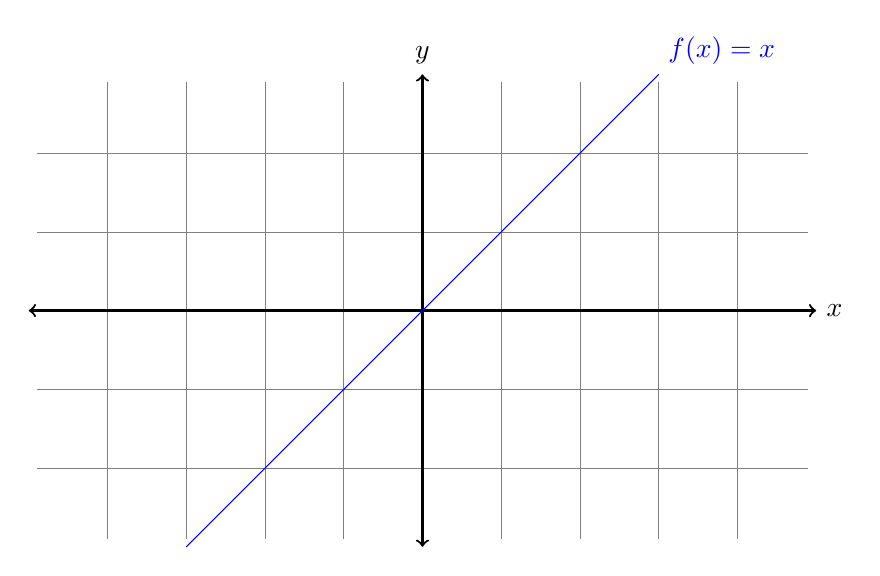
\begin{tikzpicture}
                    \draw[help lines] (-4.9,-2.9) grid (4.9,2.9);
                    \draw[black, thick, <->] (-5,0) -- (5,0) node[right]{$x$};
                    \draw[black, thick, <->] (0,-3) -- (0,3) node[above]{$y$};
                    \draw[scale=1, domain=-3:3, variable=\x, blue]  plot ({\x}, {\x}) node[above right] {$f(x) = x$};
                \end{tikzpicture}
            \end{center}
            \item[Função Linear] é aquela que quando aplicada a qualquer elemento do domínio, tem como imagem o elemento multiplicado por uma constante (coeficiente angular) diferente de 0. É construída no gráfico como uma reta que passa pela origem:
            \[ f(x) = ax \]
            \begin{center}
                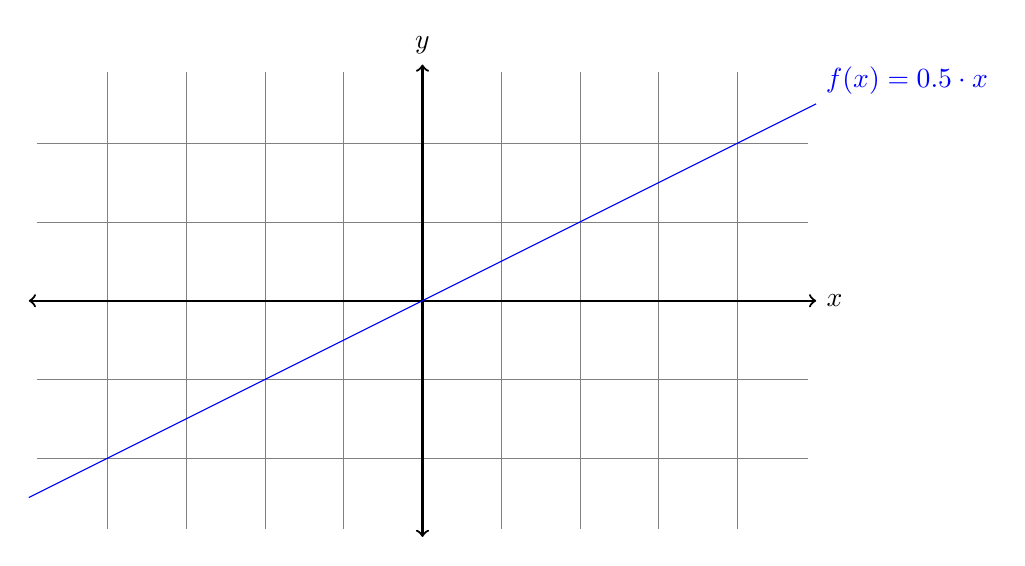
\begin{tikzpicture}
                    \draw[help lines] (-4.9,-2.9) grid (4.9,2.9);
                    \draw[black, thick, <->] (-5,0) -- (5,0) node[right]{$x$};
                    \draw[black, thick, <->] (0,-3) -- (0,3) node[above]{$y$};
                    \draw[scale=1, domain=-5:5, variable=\x, blue]  plot ({\x}, {0.5 * \x}) node[above right] {$f(x) = 0.5 \cdot x$};
                \end{tikzpicture}
            \end{center}
            \item[Função Polinomial] é aquela que tem como lei de formação uma expressão algébrica entre monômios. É classificada por grau, este que se define pelo maior expoente de sua variável:
            \[ (n \in \mathbb{N}^*), (a_n \neq 0) \]
            \[ \mathrm{P}(n) = \displaystyle\sum_{i=0}^{n} {a_{i}x^{i}} = a_{0}x^{0} + a_{1}x^{1} + ... + a_{n-1}x^{n-1} + a_{n}x^{n} \]
            \item[Função Periódica] \[ \Upsilon \pi o \mu o \nu \eta \]
            \item[Função Trigonométrica] \[ \Upsilon \pi o \mu o \nu \eta \]
            \item[Função Analítica] \[ \Upsilon \pi o \mu o \nu \eta \]
        \end{description}
    %--- 4.2.6
    \subsubsection{Graus de Funções Polinomiais}
        \begin{description}
            \item[Primeiro Grau:] chamada função afim, tem sua reta definida pelo coeficiente angular e deslocada pelo coeficiente linear:
                \[ \mathrm{P}(1) = a_{0}x^{0} + a_{1}x^{1} \]
                \[ f(x) = ax + b \]
                \begin{center}
                    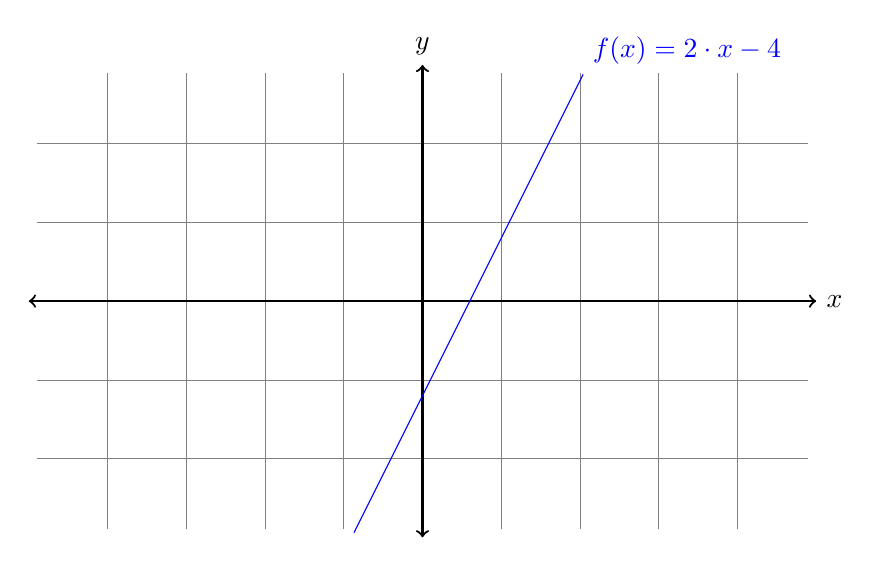
\begin{tikzpicture}
                        \draw[help lines] (-4.9,-2.9) grid (4.9,2.9);
                        \draw[black, thick, <->] (-5,0) -- (5,0) node[right]{$x$};
                        \draw[black, thick, <->] (0,-3) -- (0,3) node[above]{$y$};
                        \draw[scale=0.3, domain=-2.9:6.8, variable=\x, blue]  plot ({\x}, {2 * \x - 4}) node[above right] {$f(x) = 2 \cdot x - 4$};
                    \end{tikzpicture}
                \end{center}
                É crescente ou decrescente segundo o coeficiente angular:
                \[ (\Uparrow \ \leftrightarrow a > 0) \therefore \ (\Downarrow \ \leftrightarrow a < 0) \]
                Tem como ponto notável:
                \[ \left(\frac{-b}{a}, 0\right) \]
            \item[Segundo Grau:] chamada função quadrática, tem seu gráfico construído por uma parábola:
                \[ \mathrm{P}(2) = a_{0}x^{0} + a_{1}x^{1} + a_{2}x^{2} \]
                \[ f(x) = ax^2 + bx + c \]
                \begin{center}
                    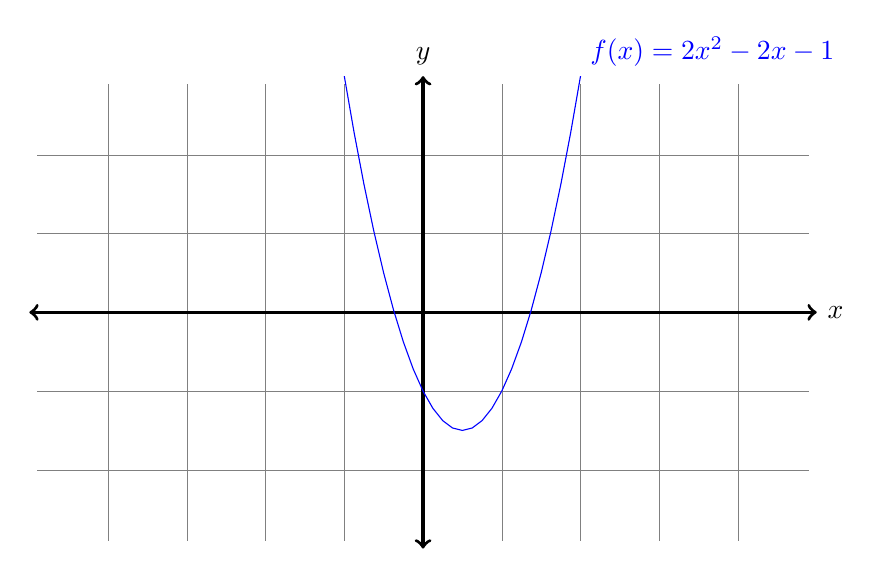
\begin{tikzpicture}
                        \draw[help lines] (-4.9,-2.9) grid (4.9,2.9);
                        \draw[black, very thick, <->] (-5,0) -- (5,0) node[right]{$x$};
                        \draw[black, very thick, <->] (0,-3) -- (0,3) node[above]{$y$};
                        \draw[scale=1, domain=-1:2, variable=\x, blue]  plot ({\x}, {2 * \x * \x - 2 * \x - 1}) node[above right] {$f(x) = 2x^2 - 2x - 1$};
                    \end{tikzpicture}
                \end{center}
                Em sua forma canônica, evidencia-se a discriminante do trinômio:
                \[ f(x) = a \left[ \left( x + \frac{b}{2a} \right)^2 - \frac{\Delta}{4a^2} \right] \]
                \[ \Delta = b^2 - 4ac \]
                O número de raízes da função é deduzível a partir da discriminante do trinômio:
                \begin{multicols}{3}
                    \noindent\[ \Delta > 0 \leftrightarrow \#R = 2 \]
                    \[ \Delta = 0 \leftrightarrow \#R = 1 \]
                    \[ \Delta < 0 \leftrightarrow \#R = 0 \]
                \end{multicols}
                A direção de abertura de sua concavidade é definida pelo primeiro coeficiente da função:
                \[ (\Uparrow \ \leftrightarrow a > 0) \therefore \ (\Downarrow \ \leftrightarrow a < 0)  \]
                Desenvolvendo sua forma canônica, encontramos formulações para facilitar a determinação das raízes da função:
                \begin{multicols}{3}
                    \noindent\[ \frac{-b \pm \sqrt{\Delta}}{2a} = \{ R_1, R_2 \} \]
                    \[ R_1 + R_2 = \frac{-b}{c} \]
                    \[ R_1 \cdot R_2 = \frac{c}{a} \]
                \end{multicols}
                Tem como pontos notáveis:
                \begin{multicols}{3}
                    \noindent\[ \left( R_1, 0 \right) \]
                    \[ P_i = \left( \frac{-b}{2a}, \frac{-\Delta}{4a} \right) \]
                    \[ \left( R_2, 0 \right) \]
                \end{multicols}
            \item[Terceiro Grau:] chamada função cúbica, tem seu gráfico construído por uma curva de dois pontos de inflexão:
                \[ \mathrm{P}(3) = a_{0}x^{0} + a_{1}x^{1} + a_{2}x^{2} + a_{3}x^{3} \]
                \[ f(x) = ax^3 + bx^2 + cx + d \]
                \begin{center}
                    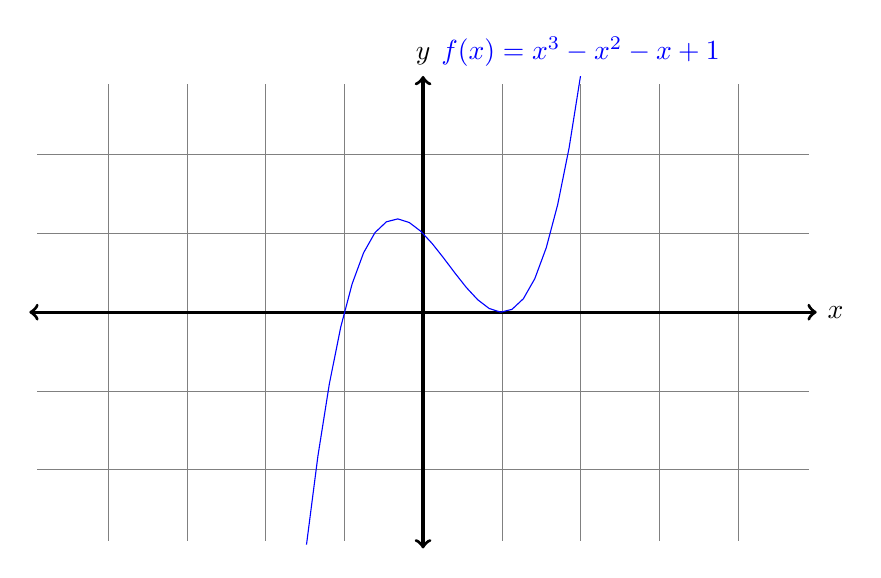
\begin{tikzpicture}
                        \draw[help lines] (-4.9,-2.9) grid (4.9,2.9);
                        \draw[black, very thick, <->] (-5,0) -- (5,0) node[right]{$x$};
                        \draw[black, very thick, <->] (0,-3) -- (0,3) node[above]{$y$};
                        \draw[scale=1, domain=-1.48:2, variable=\x, blue]  plot ({\x}, {\x * \x * \x - \x * \x - \x + 1}) node[above] {$f(x) = x^3 - x^2 - x + 1$};
                    \end{tikzpicture}
                \end{center}
                O desenvolvimento do polinômio por meio do método de Cardano-Tartaglia evidencia o discriminante da função:
                \[ \Delta = \left(\frac{ c + \frac{2a^3 - 9ab}{27}}{2}\right)^2 + \left(\frac{ b - \frac{a^2}{3}}{3}\right)^3 \]
                O número de raízes da função é deduzível a partir da discriminante da função:
                \[ \Delta > 0 \leftrightarrow \{ R_i, R_j, R_k \} \ | \ (R_i \in \mathbb{R}), (R_j, R_k \in \mathbb{C}) \]
                \[ \Delta = 0 \leftrightarrow \{ R_i, R_j, R_k \} \ | \ (R_i, R_j, R_k \in \mathbb{R}), (R_j = R_k) \]
                \[ \Delta < 0 \leftrightarrow \{ R_i, R_j, R_k \} \ | \ (R_i, R_j, R_k \in \mathbb{R}), (R_i \neq R_j \neq R_k) \]
                Usando a solução do método de Cardano-Tartaglia é possível encontrar as raízes da função:
                \[ p = \frac{c}{a} - \frac{b^2}{3a^2} \hphantom{---} q = \frac{d}{a} - \frac{bc}{3a^2} + \frac{2b^3}{27a^3}\]
                \[ R_1 = \frac{-b}{3a} + \sqrt[3]{\frac{-q}{2} + \sqrt{\left(\frac{q}{2} \right)^2 + \left(\frac{p}{3} \right)^3}} + \sqrt[3]{\frac{-q}{2} - \sqrt{{\left(\frac{q}{2} \right)^2 + \left(\frac{p}{3} \right)^3}}} \]
                \[ R_2 = \frac{-b}{3a} + \left( \frac{-1}{2} + \frac{\mathrm{i\sqrt{3}}}{2} \right) \sqrt[3]{\frac{-q}{2} + \sqrt{{\left(\frac{q}{2} \right)^2 + \left(\frac{p}{3} \right)^3}}} + \left( \frac{-1}{2} - \frac{\mathrm{i\sqrt{3}}}{2} \right) \sqrt[3]{\frac{-q}{2} - \sqrt{{\left(\frac{q}{2} \right)^2 + \left(\frac{p}{3} \right)^3}}} \]
                \[ R_2 = \frac{-b}{3a} + \left( \frac{-1}{2} + \frac{\mathrm{i\sqrt{3}}}{2} \right) \sqrt[3]{\frac{-q}{2} - \sqrt{{\left(\frac{q}{2} \right)^2 + \left(\frac{p}{3} \right)^3}}} + \left( \frac{-1}{2} - \frac{\mathrm{i\sqrt{3}}}{2} \right) \sqrt[3]{\frac{-q}{2} + \sqrt{{\left(\frac{q}{2} \right)^2 + \left(\frac{p}{3} \right)^3}}} \]
                Para além deste método, há outras ferramentas para facilitar a determinação das raízes:
                \begin{itemize}
                    \item[$\implies$] Relações de Girard:
                    \[ R_1 + R_2 + R_3 = \frac{-b}{a} \hphantom{---} R_1 \cdot R_2 \cdot R_3 = \frac{-d}{a}\]
                    \[ R_1 \cdot R_2 + R_1 \cdot R_3 + R_2 \cdot R_3 = \frac{c}{a} \]
                    \item[$\implies$] Fatoração da Equação: \[ \Upsilon \pi o \mu o \nu \eta \]
                    \item[$\implies$] Listagem de Razão Entre Fatores: \[ \Upsilon \pi o \mu o \nu \eta \]
                \end{itemize}
        \end{description}
    %--- 4.2.7
    \subsection{Interpolação Polinomial}
        \[ \Upsilon \pi o \mu o \nu \eta \]
    %--- 4.2.8
    \subsection{Divisão de Polinômios}
        \[ \Upsilon \pi o \mu o \nu \eta \]
    %--- 4.2.9
    \subsection{Fatoração de Funções Polinomiais}
        \[ \Upsilon \pi o \mu o \nu \eta \]
%------- 4.3
\subsection{Equações}
    %--- 4.3.
    \subsubsection{Equação Quadrática}
        \[ \Upsilon \pi o \mu o \nu \eta \]
    %--- 4.3.
    \subsubsection{Equação Biquadrática}
        \[ \Upsilon \pi o \mu o \nu \eta \]
    %--- 4.3.
    \subsubsection{Equação Cúbica}
        \[ \Upsilon \pi o \mu o \nu \eta \]
    %--- 4.3.
    \subsubsection{Equação Circular}
        \[ \Upsilon \pi o \mu o \nu \eta \]
%------- 4.4
\subsection{Inequações}
    %--- 4.4.1
    \subsubsection{Definição}
        Inequações são expressões algébricas de desigualdade, formando-se por sentenças matemáticas que expressam uma relação de não-equivalência entre funções:
        \[ f \star g \]
        O domínio de validade de uma inequação é a interseção dos domínios das funções, e a sua solução é dada pelo conjunto de todos os elementos do domínio de validade que cumpram a sentença de desigualdade:
        \[\mathcal{D}_{f \star g} = \mathcal{D}_f \cap \mathcal{D}_g \hphantom{---}  S_{f \star g} = \{ x \in \mathcal{D}_{f \star g} \ | \ f(x) \star g(x) \} \]
    %--- 4.4.2
    \subsubsection{Princípios de Equivalência}
        Inequações são ditas equivalentes quando possuem iguais conjuntos solução, e na resolução de uma inequação, busca-se a forma mais simples da sentença de desigualdade, tendo como referência os princípios de equivalência:
        \[ (f: \mathcal{D}_f \mapsto \mathcal{CD}_f), (g: \mathcal{D}_g \mapsto \mathcal{CD}_g), (h: \mathcal{D}_{f \star g} \mapsto \mathcal{CD}_{f \star g}) \]
        \begin{description}
            \item[P-1:] em uma inequação, podemos transpor um termo de um membro para outro trocando o sinal do termo considerado:
            \[ f + h \star g \equiv f \star g - h \]
            \[ f \star g \equiv f + h \star g + h \]
            \item[P-2:] em uma inequação, podemos multiplicar os dois membros pela mesma expressão, mantendo ou invertendo o sentido da desigualdade, conforme essa expressão seja positiva ou negativa, respectivamente:
            \[ f \ \overrightarrow{\star} \ g  \equiv \begin{dcases} f(x) \cdot h(x) \overrightarrow{\star} g(x) \cdot h(x) \leftrightarrow h(x) > 0 \\ f(x) \cdot h(x) \overleftarrow{\star} g(x) \cdot h(x) \leftrightarrow h(x) < 0 \end{dcases} \]
        \end{description}
    %--- 4.4.3
    \subsubsection{Simultâneas}
        Inequações simultâneas são a conjunção de 2 inequações alinhadas, e portanto, seu conjunto solução será a interseção do conjunto solução das inequações quando decompostas e resolvidas individualmente:
        \[ f \star g \star h \equiv \begin{dcases} f \star g \\ g \star h \end{dcases} \ \rightarrow \ S_{f \star g \star h} = S_{f \star g} \cap S_{g \star h} \]
%------- 4.5
\subsection{Sequências}
    %--- 4.5.1
    \subsubsection{Definição}
        Uma sequência é uma função onde o domínio é limitado ao conjunto dos números naturais não-nulos, assim indexando o contradomínio através da lei de aplicação e formando a imagem como uma lista ordenada. Sequências podem ser finitas ou infinitas:
        \begin{multicols}{2}
            \noindent\[ f:\mathbb{N}^i \mapsto \mathbb{R} = \{ (i, t_i) \forall i \in \mathbb{N}^i \} \]
            \[ f:\mathbb{N} \mapsto \mathbb{R} = \{ (i, t_i) \forall i \in \mathbb{N} \} \]
        \end{multicols}
    %--- 4.5.2
    \subsubsection{Lei de Formação}
        A lei de formação de uma sequência é sua lei de aplicação, e pode ser apresentada de 3 distintas formas:
        \begin{description}
            \item[Fórmula de Recorrência:] define-se o primeiro termo e a regra para encontrar seus subsequentes. \eg
            \[ f = \begin{dcases} t_1 = 1 \\ t_i = t_{i-1} + t_{i-2} \end{dcases} \forall i \in \mathbb{N} \ = \ \{1,1,2,3,5,8,13,21,...\} \]
            \item[Fórmula Geral:] a lei de aplicação expressa cada termo através de seu índice. \eg
            \[ b = \{ (i,t_i) \ | \ t_i = 2^i \ \forall i \in \mathbb{N} \} = \{2,4,8,16,32,64,128,256,...\} \]
            \item[Propriedade dos Termos:] é descrita uma propriedade que os termos devem cumprir. \eg
            \[ p = \text{todos os números primos em ordem crescente} = \{2,3,5,7,11,13,...\} \]
        \end{description}
    %--- 4.5.3
    \subsubsection{Progressão Aritmética}
        \begin{description}
            \item[Definição:] é toda sequência definida por fórmula de recorrência onde todo termo é igual ao seu antecedente somado a uma constante (razão), podendo ser classificada como crescente, decrescente ou constante em função dessa constante:
            \[ P.A. = \begin{dcases} t_1 = n \\ t_i = t_{i-1} + r \end{dcases} \ \rightarrow \ t_i = t_1 + r(i-1) \]
            \item[Interpolação Aritmética:] é inserir meios aritméticos entre dois extremos definidos, onde a razão será encontrada a partir do número de elementos interpolados:
            \[ r = \frac{t_i - t_1}{i - 1} \]
            \item[Soma dos Termos:] fórmula geral para a soma dos termos de uma progressão aritmética:
            \[ S_i = \frac{i(t_1 + t_i)}{2} \ = \ i \cdot t_1 + r \frac{i(i-1)}{2} \]
        \end{description}
    %--- 4.5.4
    \subsubsection{Progressão Geométrica}
        \begin{description}
            \item[Definição:] é toda sequência definida por fórmula de recorrência, onde todo termo é igual ao seu antecedente multiplicado por uma constante (razão), podendo ser classificada como crescente, constante, decrescente, alternante (quando os termos alternam os sinais) ou estacionária (quando a razão é zero):
            \[ P.G. = \begin{dcases} t_1 = n \\ t_i = t_{i-1} \cdot r \end{dcases} \ \rightarrow \ t_i = t_1 \cdot r^{i-1} \]
            \item[Interpolação Geométrica:] é inserir meios geométricos entre dois extremos definidos, onde a razão será encontrada a partir do número de elementos interpolados:
            \[ r = \sqrt[i-1]{\frac{t_i}{t_1}} \]
            \item[Soma dos Termos:] fórmula geral para a soma dos termos de uma progressão geométrica:
            \[ S_i = t_1 \frac{r^i -1}{r - 1} \ = \ t_i \frac{r-t_1}{r-1} \]
            \item[Produto dos Termos:] fórmula geral para o produto dos termos de uma progressão geométrica:
            \[ P_i = t_1^i \cdot r^{\frac{i(i-1)}{2}} = (t_1 \cdot t_i)^{\frac{i}{2}} \]
        \end{description}